\documentclass{article}

\usepackage{url}
\usepackage{graphicx}

\begin{document}

% Letter of transmittal
\thispagestyle{empty}
\noindent
CMU SMC 4349\\
5000 Forbes Avenue\\
Pittsburgh, PA, 15289

\vspace{2em}

\noindent
May 7, 2014

\vspace{2em}

\noindent
Mr. Thomas M. Keating\\
Assistant Teaching Professor\\
School of Computer Science\\
Pittsburgh, PA, 15289

\vspace{2em}

\noindent
Dear Mr. Keating,

\vspace{2em}

\noindent
Included with this letter is the final report for our team's project,
    ``Iron Legacy.''
     This report covers our team's approach to the project and the project
     results.

\vspace{2em}

\noindent
This report details the problem that our project addresses, 
    as well as our solution.
    The report also lists our projects goals
    and describes the technologies we used and considered.
    Finally, the report details the results and includes an evaluation of our
    team's work, the lessons we learned, and advice for future groups.

\vspace{2em}

\noindent
If you have questions about our project and wish to contact us,
    please send an email to wtwood@andrew.cmu.edu.

\vspace{2em}

\noindent
Sincerely,

\vspace{1em}

\noindent
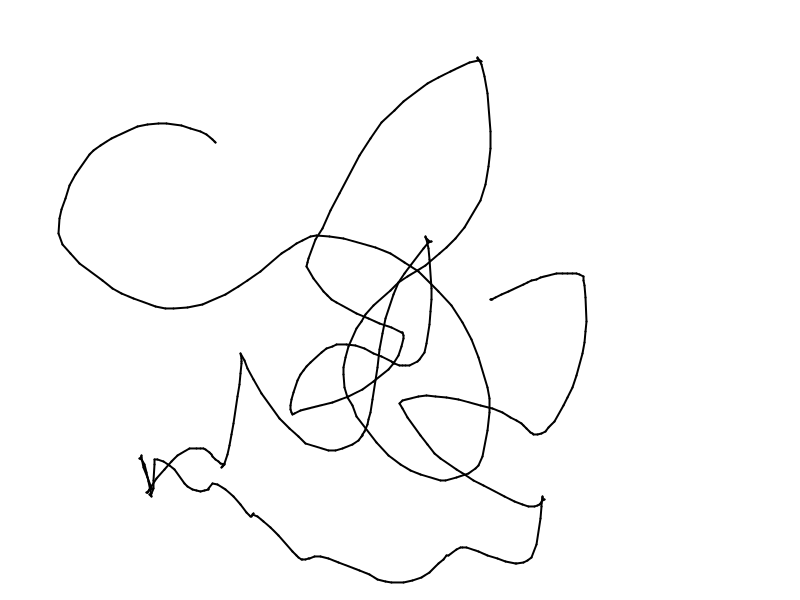
\includegraphics[height=2.5em]{Signature.png}

\vspace{0.5em}

\noindent
Billy Wood

\vfill

\noindent
enclosure: paper entitled ``Iron Legacy''

\clearpage

% Title page
\thispagestyle{empty}

\begin{center}
\bf\large
Final Report:\\
\Huge
Iron Legacy
\end{center}

\vfill

\begin{center}
\textbf{Team 9}\\
Jonathan Farr\\
Philip Garrison\\
Greg Kownacki\\
Billy Wood
\end{center}

\vfill

\begin{center}
\textbf{Submitted to}\\
Thomas M. Keating\\
Assistant Teaching Professor\\
School of Computer Science\\
Carnegie Mellon University
\end{center}

\vfill

\begin{center}
\textbf{Prepared by}\\
\begin{minipage}[c][3.7em][t]{.45\textwidth}
\begin{center}
Billy Wood\\
Mellon College of Science\\
Carnegie Mellon University
\end{center}
\end{minipage}
\begin{minipage}[c][3.7em][t]{.45\textwidth}
\begin{center}
Philip Garrison\\
Carnegie Institute of Technology\\
Carnegie Mellon University
\end{center}
\end{minipage}\\
May 7, 2014
\end{center}

\vfill

\begin{abstract}
This report describes \emph{Iron Legacy}, a turn-based strategy game that aims 
to innovate on traditional strategy game models. We created the game with 
Python and Pygame. We met weekly and used Git to collaborate. We failed to 
complete the game; most notably, it is lacking a computer AI. Because of this, 
the game is neither fun nor challenging, although it is still playable by two
people taking turns on a single computer. Due to the same time constraints that 
prevented us from completing the game, there has been no outside testing of 
\emph{Iron Legacy}. We learned valuable lessons on team organization and 
software management, which we hope future groups can learn from.
% Total: 112 words, according to google docs and wordcounter.net
\end{abstract}

\clearpage

% Table of Contents
\pagenumbering{roman}
\tableofcontents
% TODO
% Make sure sub/section names match those in the
% \addcontentsline command

\clearpage

% Introduction
\pagenumbering{arabic}
\addcontentsline{toc}{section}{Introduction}
\section*{Introduction}
This section first introduces the problem our project aims to solve and some
games similar to ours.
Then we comment on the value of the literature review and take a look at our
solution and its level of success.

\addcontentsline{toc}{subsection}{Problem}
\subsection*{Problem}
There are games that allow the player to control a units in a
small-scale battle, however these games do not give a sense of the overarching
war which leads to these battles.
Other games allow the player to control squads of units in a world-map,
however squads fight and kill each-other based on a deterministic algorithm.
Our team recognized that there is a need for a game where the player controls
battles on the both scales.

\addcontentsline{toc}{subsection}{Background}
\subsection*{Background}
We designed \emph{Iron Legacy} with the games 
\emph{Fire Emblem}$\,^1$ and \emph{Civilization}$\,^2$ 
in mind.
\emph{Fire Emblem} is recognized as one of the best games which
focuses on tactics in individual battles,
while \emph{Civilization} is praised in the genre of turn-based war strategy.

\addcontentsline{toc}{subsection}{Literature Review}
\subsection*{Literature Review}
Over the course of the project, we looked to three resources in particular:
``Towards an Evenly Match Opponent AI in Turn-based Strategy Games,''$\,^3$
a paper on adaptive-strength AI, 
``A Survey of Procedural Terrain Generation Techniques using Evolutionary 
Algorithms,''$\,^4$ a paper that helped us dynamically
generate the world map, and a forum post ``The Pixel Art 
Tutorial''$\,^5$ for creating images in the game.
In general, these were very useful.
We developed our terrain generation algorithm using an algorithm from the 
second paper, and we designed our art using the tips from the pixel art
tutorial.
The AI paper of limited use, because we did not create an AI for
the game. However, we did think that the paper was useful
as it did inform our thoughts on a potential AI design.

\addcontentsline{toc}{subsection}{Solution}
\subsection*{Solution}
Our solution is to create a strategy game in which the player will move squads
on a large-scale world-map, and spawn off micro-scale battles when two squads
collide.
This would combine the best elements of both game-styles,
thus filling the observed gap in the strategy genre.
We intended to create a fun and challenging gameplay experience by developing
an intuitive interface and a challenging computer AI.

\addcontentsline{toc}{subsection}{Success}
\subsection*{Success}
\emph{Iron Legacy} does not succeed in addressing the problem.
While the core of the game is finished, many of the features have not been
implemented.
Most notably, we did not create the AI as intended,
and without an AI, meaningful single-player gameplay is impossible.
Instead, the game is only playable by multiple players on a single computer.
Further, we had intended for squads on the world-map to influence
the micro-battles, but this feature is also unimplemented.
We will elaborate on the difficulties faced in the Results section of this
report.

Keeping our overwhelming failure in mind, we did have some limited success.
When two squads collide on the world-map, new micro-battles spawn.
All terrain is randomly generated, using one of the procedural algorithms
we discovered in our literature review.
We also created a very simple level-up system that makes units stronger
based on their most used skills.

% Approach
\addcontentsline{toc}{section}{Approach}
\section*{Approach}
The objective of this project was to build a turn-based strategy game with 
shifting-scale battles.
When two squads collided on the world-map, they would spawn a new instance of
a micro-battle.
This would appear as a battle on the world-map, and adjacent squads would be
able to send reinforcements, thus creating interactions between the two
levels of strategy.
Our four main goals were to make the game fun, challenging, strategic, and 
simple to play from a user interface perspective.

From a technical standpoint, we needed a framework in which we could write the
game logic, handle user input, and update the display in real time.
We considered the Python$\,^6$, Java$\,^7$, and 
Javascript$\,^8$ languages for writing the game. 
We settled on Python because it was the only language that we all knew
and we had some ideas of game libraries we could use.
The two libraries we looked at were Pygame$\,^9$ and TkInter$\,^{10}$.

Through Jonathan's past experience using TkInter in 15-112 and Greg's 
experience with Pygame, we chose to eschew TkInter in favor of Pygame.

For collaboration and version control, our team used Git$\,^{11}$ to
synchronize documents and code.

% Results
\addcontentsline{toc}{section}{Results}
\section*{Results}

Our project, \emph{Iron Legacy}, was unsuccessful in accomplishing
    our goals.
    The final product allows squads to move around on a macro-scale world-map.
    When squads collide, they spawn a new micro-scale battle.
    This was the intended core of the game, but the final product is lacking
    key features.

The most notable missing feature is the AI.
    The game must be played by multiple players on the same computer.
    This breaks one of the desired aspects of the game,
    namely that the world-map would run in real-time.
    Since players are on the same computer, they must take turns when making
    moves, even on the macro-scale.

We had also intended for the macro-scale to be able to influence the
    micro-scale.
    However, due to time constraints, we were unable to add this feature.
    Thus, the micro-battles and the world-map are mostly independent,
    which removes a key element of strategy that we had intended.

In our proposal, we had stated that our goal was to make a fun, challenging,
    strategic, and simple game.
    However, without an AI, it is hard to guage the ``challenge'' of our game.
    As mentioned, the strategic elements were lessened by the lack of
    interaction between the micro-battles and the world-map.
    Our game also lacks certain graphical elements, such as which squares
    can be attacked and how much health each unit has, making the interface
    confusing.

Our proposal gave very vague measures for evaluation.
    In particular, it said that ``the game must be free of all bugs that
    inhibit the natural flow of the game.''
    From there, we suggested that we would make the game publicly available,
    once it was playable.
    Last, we suggested that there should be no single-best tactic in the game,
    but that all tactics should have advantages and disadvantages.

As the game only recently reached a playable state,
    we never had the oportunity to make it publicly available.
    As such, we never received outside opinions about the quality of the game.
    Moreover, we cannot say whether any strategies are ``best,''
    as we have not collected any data from games.

Last, while the game is now playable, it is certainly not ``free of all bugs.''
    There are a few issues with the square highlighting that shows
    where a unit can move.
    Further, the game occasionally crashes when a unit is killed.
    This blatantly inhibits the natural flow of the game.

% Discussion
\addcontentsline{toc}{section}{Discussion}
\section*{Discussion}

In this section, we will discuss the lessons we learned from working 
    on a large group project.
    We will then make recommendations for how to improve \emph{Iron Legacy}.

\addcontentsline{toc}{subsection}{Lessons Learned}
\subsection*{Lessons Learned}

Our biggest lesson was the importance of meeting as a group.
    When we began discussing \emph{Iron Legacy}, the entire team was thrilled
    by the idea.
    However, we all prioritized other assignments above this game,
    and so we did not make much progress during the first month of development.
    Because we didn't have much progress, we didn't think it was worth
    getting together as a group.
    In our experience, when we did meet, we worked very productively
    and enthusiastically.
    Had we begun by scheduling a weekly meeting time,
    we probably would have stayed closer to our original Gantt chart.

We also learned the importance of designing interfaces before starting to
    program.
    As a team, we wrote code in a very \emph{ad hoc} manner.
    For instance, in writing the interface for the player to control the game,
    we put all of the logic for unit movement into the key-listener's
    event-handler.
    While this makes sense for the player, it means that the AI would have
    to press a key in order to do anything.
    This was one of the primary reasons that we never wrote AI.
    In reality, we needed to move all of the logic to separate functions that
    both the AI and the key-listener could call.
    As time went on, the task of refactoring our code to the interface model
    became increasingly intimidating, and it was never accomplished.

\addcontentsline{toc}{subsection}{Recommendations for Improvement}
\subsection*{Recommendations for Improvement}

The next step for \emph{Iron Legacy} would be AI.
    As mentioned in the lessons learned, this means refactoring a large
    chunk of the code such that there is a single interface
    of functions for the AI to call in order to control units.

After that, we would suggest making the game available in a beta-test,
    to see which features players like and dislike.
    We would like to give out a survey with quantitative
    responses in order to get hard data on which features most need
    improvement.

During future testing, we suggest gathering data on which squads
    win and lose during the micro-battles.
    This would provide quantitative data that would show if one unit
    is stronger than the others.
    From here, we could weigh the strengths and
    weaknesses of the different play-strategies, in order to make
    the game as balanced as possible.

For future groups, we adivse planning code structure before writing code,
    instead of building everything from the bottom up. We also recommend
    honestly and accurately assessing the time requirements of the project
    and the time the team will commit to the project.
\clearpage

% Sources Cited
\addcontentsline{toc}{section}{References}
\section*{References}

\noindent
$\,^1$
\emph{Fire Emblem} - {\tt http://fireemblem.nintendo.com/}

\vspace{.3em}

\noindent
$\,^2$
\emph{Civilization} - {\tt http://civilizaton.com}

\vspace{.3em}

\noindent
\hangindent=1cm
% TODO format these better
$\,^3$
Potisartra, K., \& Kotrajaras, V. Towards an Evenly Match AI in Turn-based Strategy Games. Accessed May 5, 2014. \url{http://www.cp.eng.chula.ac.th/~vishnu/gameProg/papers/CGAT_TowardsEvenlyMatchTBS-FINAL.pdf.}

\vspace{.3em}

\noindent
\hangindent=1cm
$\,^4$
Raffe, W., Zambetta, F., \& Li, X. A Survey of Procedural Terrain Generation Techniques using Evolutionary Algorithms, June 10, 2013. Accessed May 5, 2014. \url{http://goanna.cs.rmit.edu.au/~xiaodong/publications/ptg-raffe-cec2012.PDF}.

\vspace{.3em}

\noindent
\hangindent=1cm
$\,^5$
Cure. Cure to Pixel Joint web forum, "The Pixel Art Tutorial," November 27, 2010. Accessed April 8, 2014. \url{http://www.pixeljoint.com/forum/forum_posts.asp?TID=11299}. 

\vspace{.3em}

\noindent
$\,^6$
Python - {\tt http://www.python.org}

\vspace{.3em}

\noindent
$\,^7$
Java - {\tt http://www.java.com}

\vspace{.3em}

\noindent
$\,^8$
Javascript - {\tt http://developer.mozilla.org/en-US/docs/Web/JavaScript}

\vspace{.3em}

\noindent
$\,^9$
Pygame - {\tt http://www.pygame.org}

\vspace{.3em}

\noindent
$\,^{10}$
TkInter - {\tt http://wiki.python.org/moin/TkInter}

\vspace{.3em}

\noindent
$\,^{11}$
Git - {\tt http://www.github.com}

\vspace{.3em}

\clearpage

\addcontentsline{toc}{section}{Appendix}
\section*{Appendix}

\begin{center}

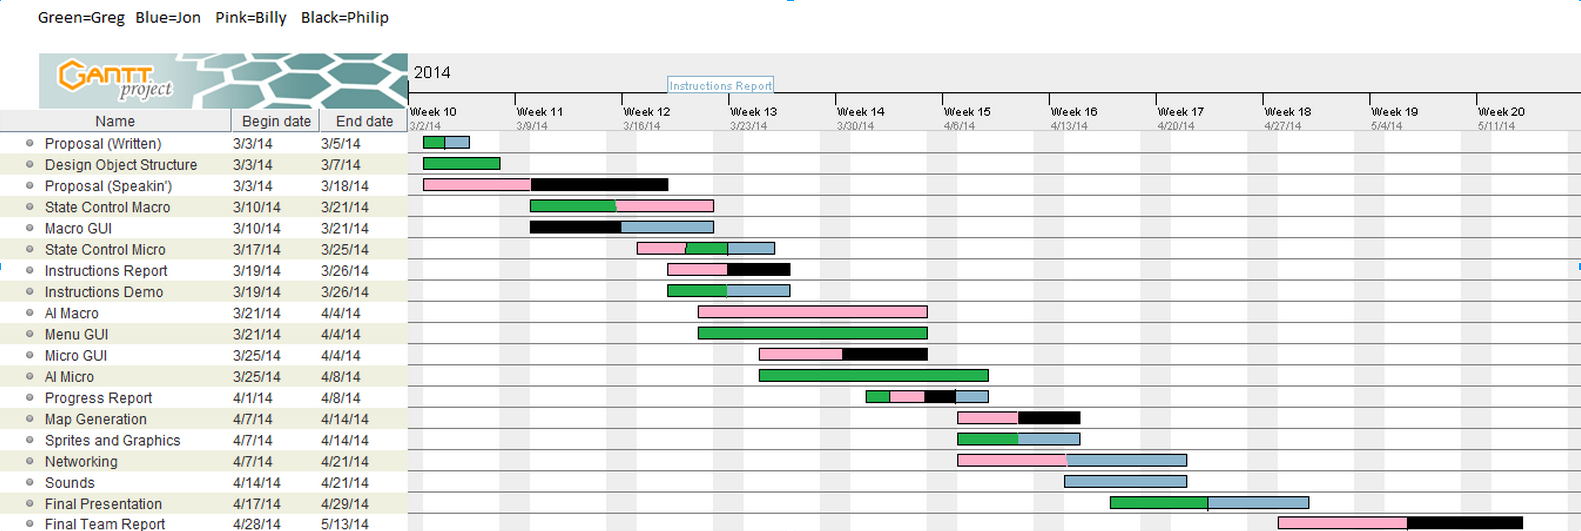
\includegraphics[width=350px]{Gantt.png}

{\bf Figure 1.} Original Gantt chart.
\end{center}


\begin{center}

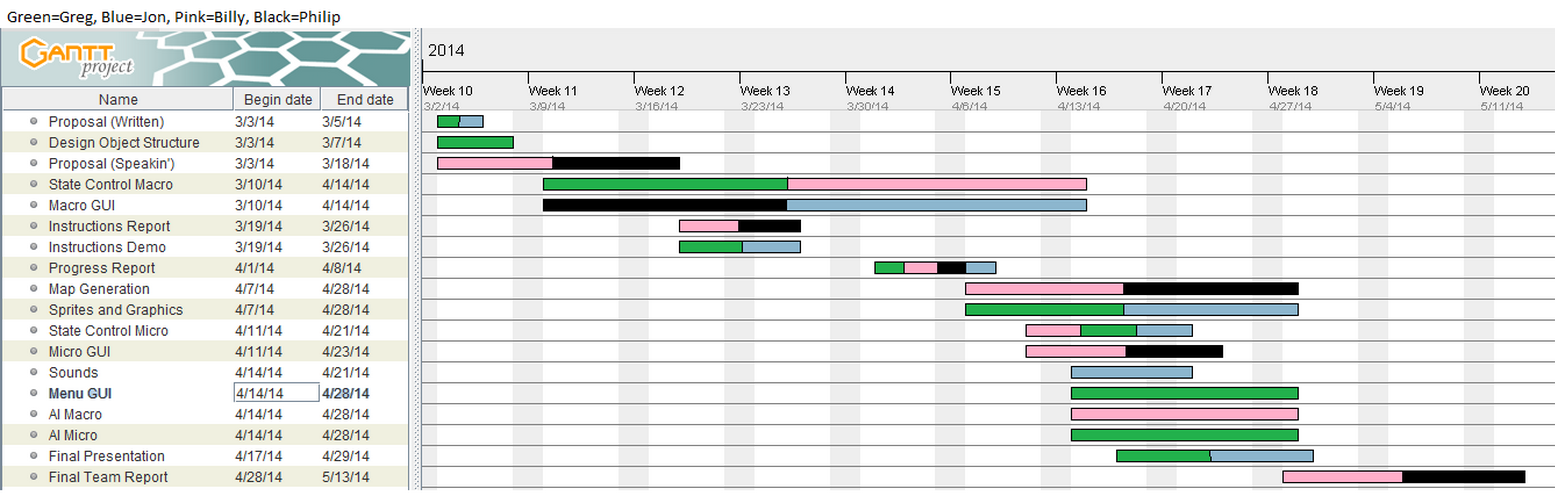
\includegraphics[width=350px]{Gantt2.png}

{\bf Figure 2.} Revised Gantt chart, as of April 8.
\end{center}

\end{document}
